\section{Backpropagation}

\subsection{Notation}

Um in einem mehrschichtigen Netz effizient die Kostenfunktion zu minimieren wird in vielen Fällen der \emph{Backpropagation}-Algorithmus verwendet. Dieser wurde bereits in den Siebzigerjahren definiert, erlangt jedoch erst im Jahr 1986 mit dem Paper \emph{Learning representations by back-propagating errors} von Rumelhart, Hinton und Williams Bekanntheit. 

Im vorherigen Teil habe ich bereits beschrieben was man unter dem Gradientenabstieg versteht und wie dieser auch bei mehrdimensionalen Funktionen (wie zum Beispiel der hierbei betrachteten Kostenfunktion) verwendet werden kann. Es wurde jedoch noch nicht vorgestellt, wie man auf ein mehrschichtiges Netz bezogen, diesen Gradienten überhaupt berechnen kann. 

Gemeinhin wird die Notation wie sie in Abbilung \ref{fig:weight_not} zu sehen ist, für ein Gewicht verwendet. In Abbildung \ref{fig:biasAct_not} steht das $b^l_j$ für den Schwellwert (\emph{Bias}) am Neuron mit dem Index \emph{j} im Layer mit dem Index \emph{l}. Selbes gilt für die Aktivierung welche mit einem \emph{a} gekennzeichnet wird. Mit den gegebenen Notationen können wir folgende Gleichung für die Aktivierung eines Neurons aufstellen (siehe Gleichung \ref{eq:act}). 

\begin{figure}[!htb]
	\centering
	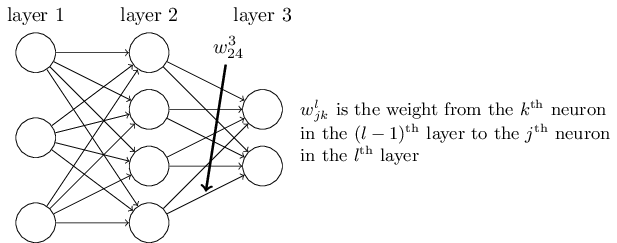
\includegraphics[width=.9\linewidth]{img/weight_notation}
	\mycaption{Notation}{dlnielsen}
	\label{fig:weight_not}
\end{figure}

\begin{figure}[!htb]
	\centering
	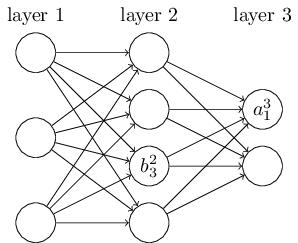
\includegraphics[width=.4\linewidth]{img/biasAct_notation}
	\mycaption{Notation}{dlnielsen}
	\label{fig:biasAct_not}
\end{figure}

\begin{equation} \label{eq:act}
a^{l}_j = \sigma\left( \sum_k w^{l}_{jk} a^{l-1}_k + b^l_j \right),
\end{equation}

Diese Formel sollte bereits aus den vorherigen Kapiteln bekannt sein. Es wird hierbei lediglich eine Vektormultiplikation der beiden eingehenden Gewichtsvektors und Addition mit den Aktivierungsvektoren durchgeführt. Die generierte Ausgabe wird mit dem Schwellwert verrechnet und in eine Aktivierungsfunktion (wie sum Beispiel der Sigmoid-Funktion) gesteckt.

Um später einfacher mit all diesen Werten zu rechnen wird versucht die gegebenen Werte in eine Matrix- beziehungsweise Vektor-Darstellungsform zu bringen. Da Neuron mehrere ausgehende \myquote{Pfade} besitzen wird hierbei eine Matrix geformt. Das bisher beschriebene Gewicht $w^l_{jk}$ befindet sich hierbei in der Zeile mit dem Index \emph{j} und Spaltenindex \emph{k}. Da sich sowohl der Schwellwert als auch die Aktivierung lediglich auf ein einzelnes Neuron beziehen muss hierfür lediglich ein eindimensionaler Vektor pro Layer \emph{l} generiert werden. Die einzelnen Komponenten werden hierbei über den Index \emph{j} angesteuert. Die Notation für den Aktivierungsvektor der Schicht \emph{l} sieht dann derartig aus: $a^l_j$. Ähnliches gilt fur die Schwellwerte: $b^l_j$. 

Um mit diesen Vektoren arbeiten zu können muss man die abschließende Aktivierungsfunktion $\sigma$ vektorisieren 
\footnote{Klarer Verweis auf Nielsen Buch, Kapitel über Backpropagation im Detail \cite{dlnielsen}}. 
Dabei muss man die Funktion lediglich derartig umschreiben, dass diese auf die einzelnen Komponenten angewendet wird und nicht auf einen einzelnen Wert. Beispielsweise würde die Funktion $f(x) = x^2$ vektorisiert folgendermaßen aussehen: 

\begin{equation}
  f\left(\left[ \begin{array}{c} 2 \\ 3 \end{array} \right] \right)
  = \left[ \begin{array}{c} f(2) \\ f(3) \end{array} \right]
  = \left[ \begin{array}{c} 4 \\ 9 \end{array} \right],
\end{equation}

Mit diesen Zusammenfassungen kann nun die Gleichung \ref{eq:act} folgendermaßen umgeschrieben werden: 

\begin{equation}
  a^{l} = \sigma(w^l a^{l-1}+b^l).
\end{equation}

Diese Umschreibung abstrahiert das Denken über die lokalen Neuronen auf ein höheres Level sodass es einfacher ist das Gesamtbild zu betrachten. Um noch mehr Klarheit zu schaffen wird oftmals die Aktivierung einer Schicht \emph{l} aus der Funktion herausgezogen und mit dem Buchstaben \emph{z} versehen. $z^l$ kann nun in die Aktivierungsfunktion $\sigma$ eingesetzt werden. Im folgenden habe ich noch einmal alle bisherigen Erkenntnisse zusammengefasst: 

\begin{mytheo}{Backpropagation - Notation}{theoexample}

Bisherige Schreibweise:
\begin{equation}
  a^{l}_j = \sigma\left( \sum_k w^{l}_{jk} a^{l-1}_k + b^l_j \right) \nonumber
\end{equation}

Zusammengefasste Form:
\begin{equation} \label{eq:zusForm}
a^l = \sigma(z^l)
\end{equation}

Gewichtete Eingabe:
\begin{equation} \label{eq:gewEin}
  z^l \equiv w^l a^{l-1}+b^l
\end{equation}

\end{mytheo}

\subsection{Fundamentale Gleichungen}

Ziel des Backpropagation Algorithmus ist es herauszubekommen welche Gewichte und Schwellwerte verändert werden müssen um die Kostenfunktion zu minimieren. Im folgenden werde ich nach und nach die vier wichtigsten Formeln des Verfahrens beschreiben. 

\begin{mytheo}{Backpropagation - Fundamentale Gleichungen}{theoexample} \label{theo:zus}

\begin{equation} \label{eq:error}
\delta^L = \nabla_a C \odot \sigma'(z^L).
\end{equation}

\begin{equation} \label{eq:recError}
\delta^l = ((w^{l+1})^T \delta^{l+1}) \odot \sigma'(z^l),
\end{equation}

\begin{equation}
\frac{\partial C}{\partial b^l_j} = \delta^l_j.
\end{equation}

\begin{equation}
\frac{\partial C}{\partial w^l_{jk}} = a^{l-1}_k \delta^l_j.
\end{equation}

\end{mytheo}


\paragraph{Fehler auf der Ausgabeschicht - Gleichung \ref{eq:error}}
Um zu verstehen was man unter einem Fehler genau versteht sei angenommen die Ausgabe eines Neurons \emph{j} im Layer \emph{l} wird um einen unbestimmten Wert verzerrt. Mathematisch ausgedrückt sieht dies dann folgendermaßen aus: 

\begin{equation}
\sigma(z^l_j+\Delta z^l_j)
\end{equation}

Statt der herkömmlichen Ausgabe $\sigma{z^l_j}$ wird ein \emph{Fehler} $\Delta z^l_j$ hinzugefügt. Allgemein wird der Fehler eines einzelnen Neurons dadurch folgendermaßen beschrieben: 

\begin{equation}
\delta^l_j \equiv \frac{\partial C}{\partial z^l_j}.
\end{equation}

Fangen wir jedoch von vorne an. Bei der Backpropagation wird versucht von den Fehlern welche am Ende auftreten auf die verschiedenen Gewichte und Schwellwerte zu schließen die verändert werden müssen. Hierbei wird zuallererst der durchschnittliche Fehler der letzten Schicht berechnet. Hierfür wird die Kostenfunktion nach dem jeweiligen normalisierten Ausgabewerts eines Neurons mit Index \emph{j} abgeleitet.

\begin{equation} \label{eq:1}
\delta^L_j = \frac{\partial C}{\partial z^L_j}
\end{equation}

Wichtig hierbei, das \emph{L} steht hierbei für den letzten (Ausgabe-) Layer. Dieser Ausdruck kann etwas verfeinert werden, indem man die Kettenregel anwendet \footnote{Der Youtuber 3blue1brown hat hierzu ein sehr gutes Video produziert welches die Zusammenhänge mit der Kettenregel verdeutlicht \cite{3b1b} (Kapitel: Backpropagation)}. Zur Erinnerung, die Kettenregel sieht folgendermaßen aus:  

\begin{equation}
\frac{d}{{dx}}\left[ {f\left( u \right)} \right] = \frac{d}{{du}}\left[ {f\left( u \right)} \right]\frac{{du}}{{dx}}
\end{equation}

Für die Vereinfachung der Gleichung \ref{eq:1} wird die Definition von \emph{z} herangezogen (siehe Gleichung \ref{eq:gewEin}). Wir erinnern uns, $a^l = \sigma(z^l)$ (siehe \ref{eq:zusForm}). \emph{z} stellt in diesem Fall den kompletten Ausgabewert des Neurons dar \emph{bevor} dieser in die Aktivierungsfunktion gesteckt wurde und berechnet sich wie schon in Gleichung \ref{eq:gewEin} gezeigt mit ${z^l \equiv w^l a^{l-1}+b^l}$. Wenn man die Kostenfunktion nun nach \emph{z} ableiten möchte muss man hierbei erst einmal die äußere mit der inneren Ableitung multiplizieren. Es entsteht folgende Gleichung: 

\begin{equation}
\delta^L_j = \sum_k \frac{\partial C}{\partial a^L_k} \frac{\partial a^L_k}{\partial z^L_j}
\end{equation}

Der hintere Term $\partial a^L_k / \partial a^L_j$

Da die Aktivierung $a^L_k$ im letzten Term lediglich vom Neuron mit dem Index \emph{k} abhängt bilden alle Summanden mit $k \neq j$ den Wert null. Es kann folglich auf die nachfolgende Gleichung geschlossen werden. (Dieses Entfallen der Summe war bereits in der Herleitung des Gradientenabstiegs zu beobachten). 

\begin{equation}
\delta^L_j = \frac{\partial C}{\partial a^L_j} \frac{\partial a^L_j}{\partial z^L_j}
\end{equation}

Da gilt, dass $a^L_j = \sigma(z^L_j)$ lässt sich der zweite Term in $\sigma'(z^L_j)$ umschreiben. 

\begin{equation}
\delta^L_j = \frac{\partial C}{\partial a^L_j} \sigma'(z^L_j)
\end{equation}

Die Formel bezieht sich momentan auf eine spezifische Komponente innerhalb der letzten Schicht, Ziel dieser Einheit ist es jedoch möglichst allgemeingültige Formeln zu finden damit der Rechner effizienter arbeiten kann. Daher wird die betrachtete Formel derartig umformuliert, dass es einen Ausgabevektor gibt welcher sämtliche Fehler der Ausgabeneuronen enthält. Auf die jeweiligen Felder kann hierbei über die jeweiligen Indizes zugegriffen werden. 

\begin{equation}
\delta^L = \nabla_a C \odot \sigma'(z^L)
\end{equation}

Dies ist auch die Darstellung wie sie Anfang des Abschnitts verwendet wurde (siehe \ref{theo:zus}). $\nabla_a C$ stellt dabei den Vektor dar dessen partielle Ableitungen $\partial C / \partial a^L_j$ entsprechen (\emph{j} ist hierbei weiterhin der Index des betrachteten Neurons innerhalb des letzten Layers). Es ist also lediglich eine andere Schreibweise für die partielle Ableitung, bezogen auf die komplette Ausgabeschicht. 

\begin{equation}
\delta^L_j = \frac{\partial C}{\partial a^L_j} \sigma'(z^L_j)
\end{equation}


Wenn wir für die Kostenfunktion wie schon in früheren Kapiteln die quadratische Kostenfunktion wählen entspricht $C = \frac{1}{2} \sum_j (y_j-a^L_j)^2$. Nach $a^L_j$ abgeleitet ergibt sich dann wiederum $\partial C / \partial a^L_j = (a_j^L-y_j)$. Die Herleitung ist sehr ähnlich zu der des Gradienten (siehe \ref{deri:grad}), hier fehlt lediglich die Iteration über die kompletten Trainingsdatensätze. Diese Ableitung kann man dann ebenfalls in die Gleichung einsetzen um ein etwas klareres Bild zu schaffen. 

\begin{equation}
\delta^L = (a^L-y) \odot \sigma'(z^L)
\end{equation}
 
 
\begin{mytheo}{Zusammenfassung}{theoexample}


Um den Fehlervektor der letzten Schicht zu bestimmen: 

\begin{equation}
\delta^L = \nabla_a C \odot \sigma'(z^L).
\end{equation}


äquivalent zu: 

\begin{equation}
\delta^L = (a^L-y) \odot \sigma'(z^L)
\end{equation}


Um die Fehler komponentenweise zu bestimmen: 

\begin{equation}
\delta^L_j = \frac{\partial C}{\partial a^L_j} \sigma'(z^L_j)
\end{equation}

\end{mytheo}






\paragraph{Rekursive Fehlererkennung - Gleichung \ref{eq:recError}}

Da wir nun die Fehler des letzten Layers kennen wird diese Erkenntnis genutzt um auf die Fehler der vorherigen Schichten zu deuten. 

Man versucht mithilfe der jeweils nächsten Schicht auf die Fehlerwerte der aktuellen Schicht zu kommen. Die Gleichung $\delta^l_j = \partial C / \partial z^l_j$ wird zu $\delta^{l+1}_k = \partial C / \partial z^{l+1}_k$ umgeformt. 


